\documentclass[12pt,fleqn]{examtst}
\usepackage{graphicx}
\usepackage{amssymb}
\usepackage{amsmath}
\usepackage{listings}
\usepackage{multirow}
\usepackage{multicol}
\usepackage{hhline}
\usepackage{booktabs}
\usepackage{url}
\usepackage{enumerate}
\usepackage{hyperref}
%% Comments

\usepackage{color}

\newif\ifcomments\commentstrue

\ifcomments
\newcommand{\authornote}[3]{\textcolor{#1}{[#3 ---#2]}}
\newcommand{\todo}[1]{\textcolor{red}{[TODO: #1]}}
\else
\newcommand{\authornote}[3]{}
\newcommand{\todo}[1]{}
\fi

\newcommand{\wss}[1]{\authornote{blue}{SS}{#1}}

\begin{document}

\newcommand{\soln}{n} %y for yes and n for no

\lstset{language=python, basicstyle=\ttfamily, breaklines=true,
  showspaces=false, showstringspaces=false, breakatwhitespace=true, texcl=true,
  escapeinside={\%*}{*)}}

\newcommand{\codeit}[1]{\texttt{\textit{#1}}}

\begin{center}
  {\large \bf COMP SCI 2ME3 and SFWR ENG 2AA4 Final Examination}\\[1ex]
  {\large \bf McMaster University}\\[1ex]
  \ifthenelse{\equal{\soln}{y}}{\large {\bf Answer Key:} Large arrow
    ($\Longleftarrow$) for correct% , small ($\leftarrow$) for partially
    % correct
  }{}
\end{center}

\medskip

\noindent
DAY CLASS, \textbf{Version 1}  \hfill Dr.~S.~Smith \\
DURATION OF EXAMINATION: 4 hours \\
MCMASTER UNIVERSITY FINAL EXAMINATION \hfill April 16, 2020

\medskip

\noindent
\rule[3 mm]{\textwidth}{0.5mm}

%\begin{minipage}[t]{1.0\textwidth}

NAME: \wss{Jay Mody}\\[1ex]

Student ID: \wss{400195508} \\[2mm]

\noindent
\rule[3 mm]{\textwidth}{0.5mm}

This examination paper includes \noofpages pages and
7 % VARIABILITY
questions. You are responsible for ensuring that your copy of the examination
paper is complete. Bring any discrepancy to the attention
of your instructor.\\

\noindent
\emph{By submitting this work, I certify that the work represents solely my own
independent efforts. I confirm that I am expected to exhibit honesty and use
ethical behaviour in all aspects of the learning process.  I confirm that it is
my responsibility to understand what constitutes academic dishonesty under the
\href{https://secretariat.mcmaster.ca/app/uploads/Academic-Integrity-Policy-1-1.pdf}
{Academic Integrity Policy}}.\\

\noindent
\textbf{Special Instructions}:

\begin{enumerate}

\item For taking tests remotely:
\begin{itemize}
\item Turn off all unnecessary programs, especially Netflix, YouTube, games like
  Xbox or PS4, anything that might be downloading or streaming.
\item If your house is shared, ask others to refrain from doing those activities
  during the test.
\item If you can, connect to the internet via a wired connection.
\item Move close to the Wi-Fi hub in your house.
\item Restart your computer, 1-2 hours before the exam. A restart can be very
  helpful for several computer hiccups.
\item Commit and push your tex file, compiled pdf file, and code files
  frequently.
\item Ensure that you push your solution (tex file, pdf file and code files)
  before time expires on the test.  The solution that is in the repo at the
  deadline is the solution that will be graded.
\end{itemize}
\item It is your responsibility to ensure that the answer sheet is properly
  completed. Your examination result depends upon proper attention to the
  instructions.
\item All physical external resources are permitted, including textbooks, calculators,
  computers, compilers, and the internet.
\item The work has to be completed individually.  Discussion with others is
  strictly prohibited.
\item Read each question carefully.
\item Try to allocate your time sensibly and divide it appropriately between the
  questions.
\item The set $\mathbb{N}$ is assumed to include $0$.
\end{enumerate}
%\end{minipage}\\

\examheader{CS2ME3/SE2AA4 \ifthenelse{\equal{\soln}{y}} {\hfill SOLUTIONS} }

\renewcommand{\labelenumi}{\Alph{enumi}.}

\newpage

%%%%%%%%%%%%%%%%%%%%%%%%%%%%%%%%%%%%%%%%%%%%%%%%%%%%%%%%%%%%%%%%%%%%%%

\question{5 marks} %tests software qualities - reusability?
The software quality of reusability influences several other qualities.  For
each of the following qualities, state whether reusability impacts it positively
or negatively and give a reason for your position: a) reliability, b)
efficiency, and c) maintainability.\\

\noindent \wss{Fill in the lists below}

\begin{enumerate}[a)]
\item Reliability
\begin{itemize}
\item Positive
\item Reusability requires that a piece of software can be reused in various
contexts. This often means that the software needs to general, covering a more
general use case. As a consequence, the software also becomes more
reliable, since it is designed to work in a wider range of use cases.
For example, python packages like numpy have been thouroughly tested, reused,
and maintained for years. As a result, we know that we can rely on it to work
when we reuse it in our own software.
\end{itemize}
\item Efficiency
\begin{itemize}
\item Negative
\item In most cases, software that is more general (reusable software is often
general) will likely be less efficient than software that is built for very
narrow and specific use cases. This is because reusable/generable software
contains a lot of overhead to cover a wider array of contexts.
\end{itemize}
\item Maintainability
\begin{itemize}
\item Positive
\item Software that is reusable will include interfaces, modules, and will
preserve seperation of concerns. All of these properties make the software
better at anticipating change, making it easier to maintain the software
(whether that is adding additional functionality of making bug fixes).

\end{itemize}
\end{enumerate}

%%%%%%%%%%%%%%%%%%%%%%%%%%%%%%%%%%%%%%%%%%%%%%%%%%%%%%%%%%%%%%%%%%%%%%

\newpage

\question{5 marks} When you insert a USB key into your computer you can read and
write to the USB key in the same way as you read and write to your hard drive. What
software engineering principles are being applied here? Please justify your
answer.\\

\noindent \wss{Fill in the itemized list below with your answers}

\begin{itemize}
\item Generality - A USB is general because it is not specific in what type
of data in can hold and acts almost the same as a hard drive. It can be used in
many different scenarios (transfer files from one machine to another,
backup files, boot a computer, install some software). In addition, a USB can
be reformated to fit many different file formats (FAT32, NTFS, MacOS) to allow
for transfer of files from a variety of operating systems.
\item Reusability - As stated above, the generality of a USB allows it to be
reused in a variety of scenarios (transfer files from one machine to another,
backup files, boot a computer, install some software).
\item Seperation of Concerns - The USB and computer transaction doesn't care
about where the data came from, or the software that built it, it simply will
hold whatever data you tell it to.
\item Usability - Almost all computers these days have a USB (type A) port. Even
if they don't, there are many various adapters and technologies that exists that
allow you to use your usb on almost any device.
\end{itemize}

%%%%%%%%%%%%%%%%%%%%%%%%%%%%%%%%%%%%%%%%%%%%%%%%%%%%%%%%%%%%%%%%%%%%%%

\newpage

\noindent
\begin{minipage}{\textwidth}
\question{5 marks}

Critique the following specification for a monitoring system for a water tank.
Use the criteria discussed in class for judging the quality of a specification
(consistent, abstract, unambiguous, etc):\\

``If the difference between the measured water level and the target fluid level is
under 5\%, then set variable top\_up\_req to True.''
~\\

\noindent \wss{Fill in the itemized list below with your answers}

\begin{itemize}
\item Ambiguous - The specification is ambiguous because it doesn't specify
whether it's 5\% relative to the target fluid level, or 5\% relative to the
measured water level.
\item Validatable - The specification is validatable because we can
arithmetically verify the outcome of the specification (unit testable).
\item Unabstract - The specification is not abstract, since the 5\% cutoff
is hard coded. A more abstract case would be: ``If the difference between the
measured water level and the target fluid level is under a certain
percentage threshold (default 5\%), then set variable top\_up\_req to True.''
\item Consistent/Clear - The specification is consistent since the cause and
consequence are clear, with no contradicting cases.
\item Complete - Assuming the specification has internal definitons for
measure water level, target fluid, and top\_up\_req, the specification is
internally complete leaving no untied ends and missing parts. Even though it
doesn't state what to do in the event that the fluid level's aren't within
5\%, we assume that we don't change the value of top\_up\_req.
\end{itemize}

\end{minipage}

%%%%%%%%%%%%%%%%%%%%%%%%%%%%%%%%%%

\newpage

\noindent The UML diagram below is used for Questions~\ref{Q_CompleteMIS},
\ref{Q_JavaCode}, \ref{Q_TestTable} and \ref{Q_LikelyChanges}.  You are not
required, or expected, to do the questions in order.  The organization of the
next sections is intended to appear rationale for grading purposes; it is fine
if you ``fake it'' and complete the parts in your preferred order.  In
particular, you will probably want to complete some test cases
(Question~\ref{Q_TestTable}) using the code \texttt{TestSeq1D.java} while you do
the implementation (Question~\ref{Q_JavaCode}).  You are encouraged to take some
time to read all of the related questions before beginning your answers.

Consider the generic UML class diagram (Figure~\ref{Fig_UML_Strategy}) for
Seq1D.  Seq1D contains a one dimensional sequence and provides the rank
function.  The rank function is defined for a given sequence of numerical or
ordinal values.  The rank of a value from the sequence is the position the value
would appear in if the list were sorted in ascending order.  For instance, the
integer data sequence 3, -5, -2, 9 has the corresponding rank values of 2, 0, 1,
3.  (As usual we start our index numbering at 0.)  In the cases of ties, where
more than one entry in the sequence, has the same value, it is not possible to
assign the ranking uniquely.  Therefore, the UML diagram uses the strategy
design pattern to allow for changing the algorithm for handling ties.  Further
details on the rank function can be found at:
\url{https://en.wikipedia.org/wiki/Ranking}.

For the ranking function to work the underlying data type T has to be sortable,
and equality needs to be defined.  Therefore, as shown in the diagram, T
implements the Comparable interface and inherits Object, respectively.

\begin{figure}[!h]
\begin{center}
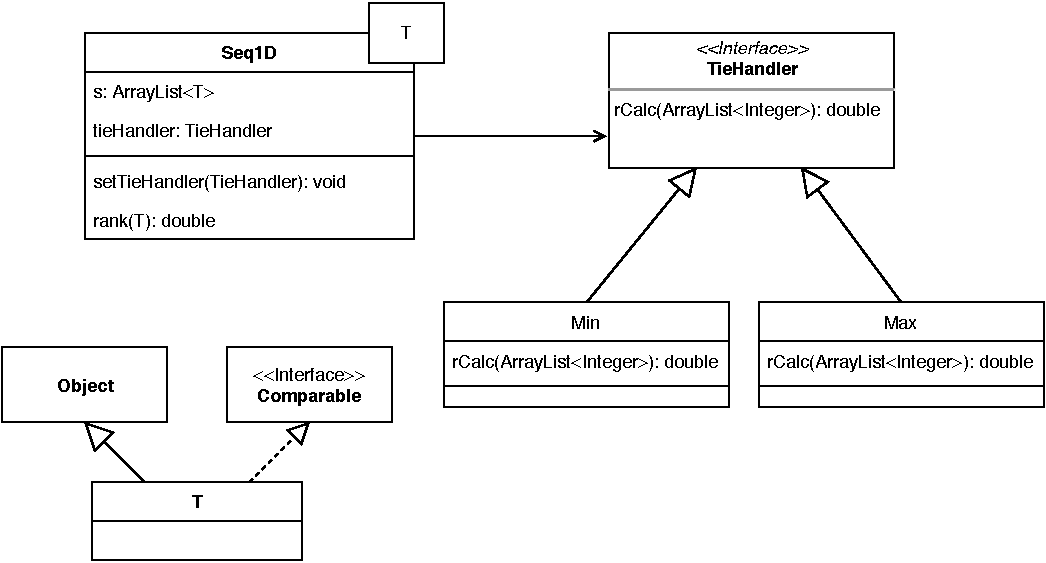
\includegraphics[scale=1]{Seq1D_StratPattern_UML.pdf}
\end{center}
\caption{Generic UML Class Diagram for Seq1D with Rank Function, using Strategy Pattern
  for Ties} \label{Fig_UML_Strategy}
\end{figure}

%%%%%%%%%%%%%%%%%%%%%%%%%%%%%%%%%%

\newpage

\noindent
\begin{minipage}{\textwidth}
\question{5 marks} \label{Q_CompleteMIS}

Over the next few pages is the corresponding MIS specification for the above UML
diagram.  Specifications for Comparable and Object are not given because they
are already available in Java.  As for A3, you should complete the specification
where indicated by comments.  (The modules that need completing are MinCalc,
MaxCalc and Seq1D).\\

\wss{The parts that you need to fill in are marked by comments, like this one.
You can use the given local functions to complete the missing specifications.
You should not have to add any new local functions, but you can if you feel it
is necessary fo your solution.}\\

\wss{As you edit the tex source, please leave the \texttt{wss} comments in the
  file.}\\

\end{minipage}

%%%%%%%%%%%%%%%%%%%%%%%%%%%%%%%%%%

\newpage

\section* {Tie Handler Interface Module}

\subsection*{Interface Module}

TieHandler

\subsection* {Uses}

None

\subsection* {Syntax}

\subsubsection* {Exported Constants}

None

\subsubsection* {Exported Types}

None

\subsubsection* {Exported Access Programs}

\begin{tabular}{| l | l | l | p{5cm} |}
\hline
\textbf{Routine name} & \textbf{In} & \textbf{Out} & \textbf{Exceptions}\\
\hline
rCalc & seq of $\mathbb{N}$ & $\mathbb{R}$ & ~\\
\hline
\end{tabular}

\subsubsection* {Considerations}

rCalc calculates the rank (a real value) from a given sequence of indices.
The order of the entries in the sequence does not matter.

%%%%%%%%%%%%%%%%%%%%%%%%%%%%%%%%%%

\newpage

\section* {Minimum Calculation for Rank with Ties Module}

\subsection*{Module inherits TieHandler}

MinCalc

\subsection* {Uses}

TieHandler

\subsection* {Syntax}

\subsubsection* {Exported Constants}

None

\subsubsection* {Exported Types}

None

\subsubsection* {Exported Access Programs}

\begin{tabular}{| l | l | l | p{5cm} |}
\hline
\textbf{Routine name} & \textbf{In} & \textbf{Out} & \textbf{Exceptions}\\
\hline
rCalc & seq of $\mathbb{N}$ & $\mathbb{R}$ & ~\\
\hline
\end{tabular}

\subsection* {Semantics}

\subsubsection* {State Variables}

None

\subsubsection* {State Invariant}

None

\subsubsection* {Assumptions}

None

\subsubsection* {Access Routine Semantics}

rCalc($s$)
\begin{itemize}
\item output: \wss{The minimum element in s, where s is a sequence of natural
    numbers} \\
    $\exists \ i : s \ .\ (\forall \ j : s \ .\ s[i] >= s[j]) \Rightarrow out := s[i]$
\item exception: none
\end{itemize}

%%%%%%%%%%%%%%%%%%%%%%%%%%%%%%%%%%

\newpage

\section* {Maximum Calculation for Rank with Ties Module}

\subsection*{Module inherits TieHandler}

MaxCalc

\subsection* {Uses}

TieHandler

\subsection* {Syntax}

\subsubsection* {Exported Constants}

None

\subsubsection* {Exported Types}

None

\subsubsection* {Exported Access Programs}

\begin{tabular}{| l | l | l | p{5cm} |}
\hline
\textbf{Routine name} & \textbf{In} & \textbf{Out} & \textbf{Exceptions}\\
\hline
rCalc & seq of $\mathbb{N}$ & $\mathbb{R}$ & ~\\
\hline
\end{tabular}

\subsection* {Semantics}

\subsubsection* {State Variables}

None

\subsubsection* {State Invariant}

None

\subsubsection* {Assumptions}

None

\subsubsection* {Access Routine Semantics}

rCalc($s$)
\begin{itemize}
\item output: \wss{The maximum element in s, where s is a sequence of natural
    numbers} \\
    $\exists \ i : s \ .\ (\forall \ j : s \ .\ s[i] <= s[j]) \Rightarrow out := s[i]$
\item exception: none
\end{itemize}

%%%%%%%%%%%%%%%%%%%%%%%%%%%%%%%%%%

\newpage

\section* {Generic Seq1D Module}

\subsection* {Generic Template Module}

Seq1D(T with Comparable(T))

\subsection* {Uses}

Comparable, TieHandler

\subsection* {Syntax}

\subsubsection* {Exported Types}

\wss{What goes here?} \\
Seq1D(T) = ?

\subsubsection* {Exported Constants}

None

\subsubsection* {Exported Access Programs}

\begin{tabular}{| l | l | l | p{6cm} |}
\hline
\textbf{Routine name} & \textbf{In} & \textbf{Out} & \textbf{Exceptions}\\
\hline
new Seq1D & seq of T, TieHandler & Seq1D & \\
\hline
setTieHandler & TieHandler &  & \\
\hline
rank & T & $\mathbb{R}$ & IllegalArgumentException\\
\hline

\end{tabular}

\subsection* {Semantics}

\subsubsection* {State Variables}

$s$: seq of T\\
tieHandler: TieHandler

\subsubsection* {State Invariant}

None

\subsubsection* {Assumptions}

\begin{itemize}
\item The Seq1D(T) constructor is called for each object instance before any
other access routine is called for that object.  The constructor can only be
called once.
\end{itemize}

\subsubsection* {Access Routine Semantics}

new Seq1D($S$):
\begin{itemize}
\item transition: $s := S$
\item output: $\mathit{out} := \mathit{self}$
\item exception: none
\end{itemize}

\noindent setTieHandler($t$):
\begin{itemize}
\item transition: $\mbox{tieHandler} := t$
\item exception: none
\end{itemize}

\noindent rank($p$):
\begin{itemize}
\item output: \wss{Calculate the rank of $p$ in the sequence, taking into
    account if there are ties} \\
    $out := \mbox{t.rCalc}(\mbox{indexSet}(p, \mbox{sort}(s)))$
\item exception: \wss{A $p$ value is illegal if it does not appear in the
    sequence} \\
    $exc := \lnot (p \in s) \Rightarrow IllegalArgumentException$
\end{itemize}

\subsection*{Local Functions}

\noindent $\mbox{indexSet}(i, B): T \times \mbox{seq of T}  \rightarrow \mbox{ set of }
\mathbb{N}$\\
\noindent $\mbox{indexSet}(i, B) \equiv \{j: \mathbb{N} | j \in [0..|B|-1]
\wedge B[j] = i : j \}$\\

\noindent $\mbox{sort}(A): \mbox{seq of } T \rightarrow \mbox{seq of T}$\\
\noindent $\mbox{sort}(A) \equiv B: \mbox{set of T}, \mbox{ such that }$\\
\noindent
$\forall (a: \mathbb{N} | a \in A : \exists(b: \mathbb{N} | b \in B: b = a)
\wedge \mbox{count}(a, A) = \mbox{count}(b, B)) \wedge \forall (i: \mathbb{N} |
i \in [0..|A|-2] : B[i] \leq B[i+1])$\\

\noindent $\mbox{count}(a, A): T \times \mbox{seq of T} \rightarrow \mathbb{N}$\\
\noindent $\mbox{count}(a, A): + (x: \mathbb{N} | x \in A \wedge x = a : 1)$\\

\noindent $\mbox{toSeq}(A): \mbox{set of } \mathbb{N} \rightarrow \mbox{seq of }
\mathbb{N}$\\
\noindent $\mbox{toSeq}(A) \equiv < i: \mathbb{N} | i \in A : i > $

\subsubsection* {Considerations}

Implementation using Java means an equals method is available.  In some cases it
may be necessary to override the Java provided equals method.

%%%%%%%%%%%%%%%%%%%%%%%%%%%%%%%%%%

\newpage

\noindent
\begin{minipage}{\textwidth}
\question{5 marks} \label{Q_JavaCode}

\wss{Complete Java code to match the above specification.}  The files you need
to complete are: \texttt{TieHandler.java}, \texttt{MinCalc.java},
\texttt{MaxCalc.java}, and \texttt{Seq1D.java}.  A testing file is also
provided: \texttt{TestSeq1D.java}.  The testing file itself isn't graded, but
creating test cases will improve your confidence in your solution.  The stubs of
the necessary files are already available in your \texttt{src} folder.  The code
will automatically be imported into this document when the \texttt{tex} file is
compiled.  You should use the provided Makefile to test your code.  You will NOT
need to modify the Makefile.
The given Makefile will work, without errors, from the initial state of your
repo.  The required imports are already given in the code.  You should not make
any modifications in the provided import statements.  You should not delete the
ones that are already there.  Although you can solve the problem without adding
any imports, if your solution requires additional imports, you can add them.  As
usual, the final test is whether the code runs on mills.

You do not need to explicitly inherit Object in Java, and you don't need to
implement the Comparable interface.  Any exceptions in the specification have
names identical to the expected Java exceptions; your code should use exactly the
exception names as given in the spec.

You do not need to worry about doxygen comments.  However, you should include
regular comments in the code in cases where the person marking would benefit
from an explanation.

Remember, your code needs to implement the given specification so that the
interface behaves as specified.  This does NOT mean that the local functions
need to all be implemented, or that the types used internally to the spec need
to be implemented exactly as given.  If you do implement any local functions,
please make them private.\\

\end{minipage}

\newpage

\subsection*{Code for TieHandler.java}

\noindent \lstinputlisting[language = Java]{./src/TieHandler.java}

\newpage

\subsection*{Code for MinCalc.java}

\noindent \lstinputlisting[language = Java]{./src/MinCalc.java}

\newpage

\subsection*{Code for MaxCalc.java}

\noindent \lstinputlisting[language = Java]{./src/MaxCalc.java}

\newpage

\subsection*{Code for Seq1D.java}

\noindent \lstinputlisting[language = Java]{./src/Seq1D.java}

\newpage

%%%%%%%%%%%%%%%%%%%%%%%%%%%%%%%%%%

\question{5 marks} \label{Q_TestTable}

Fill in the table below with 8 tests cases for the rank function, with T =
Integer.  You are only given 8 cases, so you need to select cases that are most
likely to uncover errors.  Each test case is summarized by the following:
\textbf{s} for the state of the sequence, \textbf{tie} to identify which
strategy is being used (either min or max), \textbf{p} the integer input for the
rank function, \textbf{Expected} for the expected output (either an integer or
exception), and \textbf{Explanation} to explain why you selected this particular
test case.  The explanation should identify the specific test case selection
strategy employed.  The strategy can be either white box (like statement
coverage, edge coverage etc), or black box, or stress testing, etc.  Following
the table, explain why other test cases were excluded from your short list.  What
other tests could you have done, and what is your rationale for not emphasizing
them.  Your test cases should only focus on correctness, not performance.

Although it is not technically graded, you are highly recommended to complete
the file \texttt{TestSeq1D.java} for testing \texttt{Seq1D.java} using the test
cases in your table.  More test cases in the \texttt{TestSeq1D.java} file are
fine.  The stub for \texttt{TestSeq1D.java}, and associated Makefile, are already available in
your repo.\\

\wss{Fill in this table.}\\

\textbf{NOTE: Table on next page}


\noindent
\begin{minipage}{\textwidth}

\textbf{NOTE: The table was being cutoff when I used IllegalArgumentException
under Expected, so inplace I shortened it to IllArgExc}.\\

\begin{tabular}{ p{0.75cm}  l  l  l  l p{9cm} }
  \toprule
  \textbf{\#} & \textbf{s} & \textbf{tie} & \textbf{p} & \textbf{Expected} & \textbf{Explanation}\\
  \midrule
  1 & \{\} & min & 0 & IllArgExc & Since the sequence is empty,
  any call of the rank function should return an IllegalArgumentException.
  This is an edge case where we want the rank function to fail gracefully.\\ \\
  2 & \{1,3,9\} & max & -3 & IllArgExc & Sometimes functions that
  deal with Integers will take absolute values (or cast to unsigned ints) so to
  be safe, I test that it doesn't equate -3 with 3.\\ \\
  3 & \{-100\} & min & -100 & 0 & A common edge case occurs at the lowest non-
  null value, so here I test that the function works with a single valued
  sequence. We also want to make sure that with just one element equaling p,
  MinCalc returns the correct result.\\ \\
  4 & \{-100\} & max & -100 & 0 & Same reasoning as above, but with a
  max tie handler.\\ \\
  5 & \{1,1,1,1,1,1,1,1\} & min & 1 & 0 & For rank, we typically expect a
  sequence of seemingly random integers with a couple of duplicates. We don't
  typically expect a situation where all elements are the same. We want to ensure
  that this edge case doesn't break on MinCalc, and will return 0.\\ \\
  6 & \{1,1,1,1,1,1,1,1\} & max & 1 & 7 & Same reasoning as above, but with a
  max tie handler.\\ \\
  7 & \{3,-2,-2,-5,9,9,9\} & min & 9 & 4 & This test case mimicks a more ''typical''
  case where there are duplicates and an unsorted input. So, we test it in a
  situation where we want to find the rank of a duplicate using a min tie handler.\\ \\
  8 & \{3,-2,-2,-5,9,9,9\} & max & -2 & 2 & Same reasoning as above, but with a
  max tie handler.\\ \\
  \bottomrule
\end{tabular}\\
\medskip
\end{minipage}

\clearpage
\wss{Explain below why other tests were left out.}\\
\begin{itemize}
    \item I left out test cases for longer sequences with more duplicates and
    integers because a test case with the same complexity with fewer examples
    are much easier to test for and will cover the same logical
    bugs/functionality (exclusing things like performance, efficiency,
    resource use, etc ...).

    \item In addition, I left out a test case where the array is already sorted,
    since I used the Collections library and the Comparable Integer (which
    are already rigourosly tested and valid).

    \item I also left out a test case for an array where no duplicates exist,
    as I felt that most of the possible bugs for that situation are covered by
    the other test cases as a whole (although I did test for that in my JUnit
    unit testing module, just didn't include it here).
\end{itemize}

%%%%%%%%%%%%%%%%%%%%%%%%%%%%%%%%%%

\newpage

\noindent
\begin{minipage}{\textwidth}
\question{5 marks} \label{Q_LikelyChanges}

\begin{enumerate}[a.]
\item Another strategy for handling ties in the rank function is to average the
  natural numbers in the index set, rather than finding the minimum or maximum.
  What changes to \texttt{Seq1D.java} do you need to make to use the average
  strategy?  Would you have to define any additional classes?  If yes, describe
  what would be involved in writing this new code; you do not need to provide
  the actual code.
\item In the test cases above, you have used type T = Integer, but since the
  specification is written generically other types could be used.  Assume that
  we want to add a type for students, say \texttt{StudentT}, what changes are
  necessary to the existing Java code you have written to use this new type?
  Are there any methods that \texttt{StudentT} needs to provide?  If so, what
  are they?
\item The design for Seq1D uses an object oriented approach.  How would the
  interface for Seq1D change if you were to adopt a functional programming
  approach instead?  To answer this question provide below your revised details
  for the Exported Access Programs and State Variables.
\end{enumerate}

\noindent{Fill in the itemized list below}

\begin{enumerate}[a.]
\item \wss{Your answer here.} \\
We could define an additional class called AvgCalc that also implements
TieHandler where rCalc would output the average between the max and min values
of the sequence of integers. Average here is ambiguous, as it could mean the
mean value, median value, mode value, or some other variation of an average.
No changes would need to be made to Seq1D (or any other class other than the new
one).

\item \wss{Your answer here.} \\
With my given implementation, as long as StudentT extends Comparable (in other
words, it has a valid compareTo function), no other necessary changes would need
to be made. We could change the way Seq1D works, where inplace of having the generic
type T be comparable, we have the client pass in a Comparator that compares type T,
but this is not the case as the UML specified that T extended Comparable.

\item \wss{Revise the following portions of the syntax section of the
    functional programming version of Seq1D.  The spec given is for the OO
    version.  You can make any changes you feel are necessary. }

\subsubsection* {Exported Access Programs}

\begin{tabular}{| l | l | l | p{6cm} |}
\hline
\textbf{Routine name} & \textbf{In} & \textbf{Out} & \textbf{Exceptions}\\
\hline
new Seq1D & seq of T, TieHandler & Seq1D & \\
\hline
setTieHandler & TieHandler &  & \\
\hline
rank & T & $\mathbb{R}$ & IllegalArgumentException\\
\hline

\end{tabular}

\subsubsection* {State Variables}

$s$: seq of T\\
tieHandler: TieHandler

\end{enumerate}
\end{minipage}

%%%%%%%%%%%%%%%%%%%%%%%%%%%%%%%%%%

\end{document}
